\section{Creating a scheduler using \texttt{SysTick} }
The next step is creating a simple scheduler that can run periodic tasks. There are three different tasks the scheduler
should execute; blink a red, a yellow and a green LED for a given period after a 
given delay in ticks. Table \ref{tab:led_schedule} lists the requirements for these tasks.

\begin{table}[H]
    \centering
    \begin{tabular}{|c|c|c|}
        \hline
         & \textcolor{darkpink}{\textit{Toggle Period}} & \textcolor{darkpink}{\textit{Initial Delay}}\\
        \hline
        \textit{Red} & 200 & 100 \\
        \hline
        \textit{Yellow} & 500 & 200 \\
        \hline
        \textit{Green} & 750 & 300 \\
        \hline
    \end{tabular}
        
    \label{tab:led_schedule}
    \caption{Requirements blinking LEDs in Ticks}
\end{table}

The code that will be presented in Subsection \ref{subsec:schedule_task} is actually all located in the same file, namely \texttt{main.c}.
However, for the sake of clarity to the reader the code is split up into different listings which makes it easier to understand what piece of code is for what reason present.

\subsection{Scheduling Tasks}
\label{subsec:schedule_task}

Different tasks have different characteristics. Some housekeeping is required to map those characteristics to different functions (the behaviour a task is executing).
Those housekeeping goes into what's called a Task Control Block (TCB) \cite{SROS}, \cite{usosii}.
This TCB is defined in Listing \ref{lst:def_scheduler} at Line \ref{line:OS_tcb}.
Characteristics of a task is the function it executes (usually a pointer pointing to the function definition), the period time this function should be called, the amount of time it waits untill it is ready to be woken up and execute the function again as the new period arose and a state.
This state is defined in Line \ref{line:OS_state}.
Usually there are three states which is \texttt{STATE\_READY}, \texttt{STATE\_WAITING} and \texttt{STATE\_RUNNING} \cite{SROS}, \cite{usosii}.
Because this scheduler is almost too simple only \texttt{STATE\_READY} and \texttt{STATE\_WAITING} are necessary.

\begin{lstlisting}[style=CStyle, caption={Definition code where a state datatype and housekeeping datatype for tasks is made}, captionpos=b, label={lst:def_scheduler}, escapechar=@]
#include <stdint.h>
#include <stddef.h>
#include <stdlib.h>
#include "register_def.h"

#include "inc\hw_memmap.h"
#include "inc\hw_gpio.h"
#include "inc\hw_apps_rcm.h"
#include "inc\hw_ocp_shared.h"

#include "blinky_tasks.h"

typedef enum
{
    STATE_READY = 0,
    STATE_WAITING
} OS_state; @\label{line:OS_state}@

typedef struct
{
    void (*task_function)(void);
    uint32_t tick_period;
    uint32_t ticks_used;
    OS_state state;
} OS_tcb;   @\label{line:OS_tcb}@

/* Global variables*/
OS_tcb tasks[8]; @\label{line:tasks_array}@
size_t amount_tasks = 0; @\label{line:amount_tasks}@
\end{lstlisting}

There are two global variables used in other parts within the same file.
\texttt{tasks} (Line \ref{line:tasks_array}) is an array that has space for 8 \texttt{OS\_tcb} objects which means a maxmimum of 8 tasks are schedulable by this scheduler unless a programer changes this number.
\texttt{amount\_tasks} keeps track howmuch stores \texttt{OS\_tcb} objects are in the \texttt{tasks} array.

\newpage
Tasks should be able to be added to the system and being executed via the scheduler.
That is exactly what the functions \texttt{OS\_add\_task()} and \texttt{OS\_run\_ready\_tasks()} do respectively (Listing \ref{lst:task_control_functions}).
The parameters related to a task are set in the global array \texttt{tasks}.
After the last parameter (which is state) is set the \texttt{amount\_tasks} global variable is incremented so the next time the function \texttt{OS\_add\_task()} is called it will set the parameters in the correct index.

\texttt{OS\_run\_ready\_tasks()} loops through the list of \texttt{tasks} starting at index 0 untill index \texttt{amount\_tasks}.
If a task has the state \texttt{STATE\_READY} then its function pointer is being called and once the function returns its state is set to \texttt{STATE\_WAITING}.
The \texttt{SysTickHandler} explained in a moment will make sure the task its state is set to \texttt{STATE\_READY} if needed.
\begin{lstlisting}[style=CStyle, caption={Task controllers}, captionpos=b, label={lst:task_control_functions}, escapechar=@]
void OS_add_task(void (*task_function)(void), uint32_t tick_period, uint32_t ticks_init_delay)
{
    tasks[amount_tasks].task_function = task_function;
    tasks[amount_tasks].tick_period = tick_period;
    tasks[amount_tasks].ticks_used = ticks_init_delay;
    tasks[amount_tasks++].state = STATE_WAITING;        @\label{line:sched_inc_tasks}@
}

void OS_run_ready_tasks()
{
    for(size_t idx = 0; idx != amount_tasks; idx++)
    {
        if(tasks[idx].state == STATE_READY)
        {
            (*tasks[idx].task_function)();
            tasks[idx].state = STATE_WAITING;
        }
    }
}
\end{lstlisting}

The \texttt{SysTickHandler()} decrements the \texttt{ticks\_used} member variable of a task (Listing \ref{lst:scheduler_systick}).
If \texttt{ticks\_used} is equal to 0 and the current state is \texttt{STATE\_WAITING} then the task has been waiting enough and the state is set to \texttt{STATE\_READY}.
The \texttt{ticks\_used} variable is set to its period so underflow is prevented (and so is invoking UB).

\begin{lstlisting}[style=CStyle, caption={Scheduler SysTick}, captionpos=b, label={lst:scheduler_systick}, escapechar=@]
void SystickHandler()
{
    for(size_t idx = 0; idx != amount_tasks; idx++)
    {
        tasks[idx].ticks_used -= 1;
        if(tasks[idx].ticks_used == 0)
        {
            if(tasks[idx].state == STATE_WAITING)
                tasks[idx].state = STATE_READY;
            tasks[idx].ticks_used = tasks[idx].tick_period;
        }
    }
}
\end{lstlisting}

The reader should now be able to see how the \texttt{state} member variable of \texttt{OS\_tcb} is used both in Listing \ref{lst:task_control_functions} and in Listing \ref{lst:scheduler_systick} in different contexts.
This \texttt{state} member variable is used as Inter Process Communication (IPC) between the event handler and the foreground program.
It makes sure the scheduler executes the correct tasks and the event handler wakes up the correct tasks if neccesary.

\newpage

The entry point for the main application is Line \ref{line:systick_sched_entry} in Listing \ref{lst:scheduler_systick_main}.
The first part of the code in Listing \ref{lst:scheduler_systick_main} has already been explained. It won't be repeated in this subsection.
For an explanation about the GPIO initialisation which is Line \ref{line:systick_sched_2} up to and including Line \ref{line:systick_sched_2} see Subsection \ref{subsec:led_drm}.
For an explanation about the \texttt{SysTick} module initialisation see Subsection \ref{subsec:systick_drm}.
If one looks at the given specification for the red LED, yellow LED and green LED in Table \ref{tab:led_schedule} the creation of the three tasks in Line \ref{line:systick_add_red}, Line \ref{line:systick_add_yellow} and Line \ref{line:systick_add_green} should make sense.
The initial delay column of Table \ref{tab:led_schedule} are passed as constants in the third argument to \texttt{OS\_add\_task()}.
The function pointers are passed via the first argument to \texttt{OS\_add\_task()}. Those functions are defined in \texttt{blinky\_tasks.c} and will be described in Subsection \ref{subsec:blinky_led}.
The second parameter is the period of the to be created task.
Those are defined using the \texttt{\#define} preprocessor directive in \texttt{blinky\_tasks.h}.
The foreground process always calls \texttt{OS\_run\_ready\_tasks()}. As long as there are tasks ready to be executed they will be called.
If there are no tasks ready at a certain point in time then the the loop will be infinitely executed searching infinitely long for a task that is ready to be executed.

\begin{lstlisting}[style=CStyle, caption={Entry point for the scheduler foreground process}, captionpos=b, label={lst:scheduler_systick_main}, escapechar=@]
int main(void)  @\label{line:systick_sched_entry}@
{

    HWREG(ARCM_BASE + APPS_RCM_O_GPIO_A_CLK_GATING) = 0x01;         @\label{line:systick_sched_1}@

    HWREG(OCP_SHARED_BASE + OCP_SHARED_O_GPIO_PAD_CONFIG_9) = 0x60;
    HWREG(OCP_SHARED_BASE + OCP_SHARED_O_GPIO_PAD_CONFIG_10) = 0x60;
    HWREG(OCP_SHARED_BASE + OCP_SHARED_O_GPIO_PAD_CONFIG_11) = 0x60;

    HWREG(GPIOA1_BASE + GPIO_O_GPIO_DIR) = 0x0E;
    HWREG(GPIOA1_BASE + GPIO_O_GPIO_DATA + (0x0E << 2)) = 0x00;     @\label{line:systick_sched_2}@

    HWREG(NVIC_ST_CTRL) = 0x00;         /* Disable SysTick during setup */  @\label{line:systick_sched_3}@
    HWREG(NVIC_ST_RELOAD) = 79999;      /* 80 000 reload value (1000p/s interrupt) */
    HWREG(NVIC_ST_CURRENT) = 0x00;      /* Clear any flags and set current value to 0 */
    HWREG(NVIC_ST_CTRL) = 0x07;         /* Enable SysTick, Enable interrupt, CLK_SRC = System clock */  @\label{line:systick_sched_4}@

    OS_add_task(blinky_red, RED_PERIOD, 100);           @\label{line:systick_add_red}@
    OS_add_task(blinky_yellow, YELLOW_PERIOD, 200);     @\label{line:systick_add_yellow}@
    OS_add_task(blinky_green, GREEN_PERIOD, 300);       @\label{line:systick_add_green}@

    while(1)
        OS_run_ready_tasks();

    return 0;
}
\end{lstlisting}

\subsection{Blinky LED}
\label{subsec:blinky_led}

The second part of the compiled code is related to the task.
Creating tasks and executing tasks is explained in the previous subsection.
This subsection describes the three functions of the three tasks that are called each time a task is executed.
The code is not complex at all but for the sake of completeness it is briefly described.

\texttt{blinky\_tasks.h} contains the function prototyping for the functions that a task is executing with the period for the tasks. This can be seen in Listing \ref{lst:blinkytask_h}. Using the preprocessor \texttt{\#define} directive makes it easy to change the period on a single place.

\begin{lstlisting}[style=CStyle, caption={\texttt{blinky\_tasks.h} prototyping the functions tasks should be called and their period}, captionpos=b, label={lst:blinkytask_h}, escapechar=@]
#ifndef BLINKY_TASKS_H_
#define BLINKY_TASKS_H_

#define RED_PERIOD      200
#define YELLOW_PERIOD   500
#define GREEN_PERIOD    750

void blinky_red(void);
void blinky_yellow(void);
void blinky_green(void);

#endif /* BLINKY_TASKS_H_ */

\end{lstlisting}

The implementation of the functions is not exciting.
In fact, all the functions are actually one-liners (see Listing \ref{lst:toggle_leds_systick_sched}).
They set another bit pattern to the red LED, yellow LED and the green LED.

\begin{lstlisting}[style=CStyle, caption={Toggling LED tasks according to Table \ref{tab:led_schedule} }, captionpos=b, label={lst:toggle_leds_systick_sched}, escapechar=@]
#include "register_def.h"

#include "inc\hw_memmap.h"
#include "inc\hw_gpio.h"
#include "inc\hw_apps_rcm.h"
#include "inc\hw_ocp_shared.h

void blinky_red(void)
{
    HWREG(GPIOA1_BASE + GPIO_O_GPIO_DATA + (0x02 << 2)) ^= 0x02;
}

void blinky_yellow(void)
{
    HWREG(GPIOA1_BASE + GPIO_O_GPIO_DATA + (0x04 << 2)) ^= 0x04;
}

void blinky_green(void)
{
    HWREG(GPIOA1_BASE + GPIO_O_GPIO_DATA + (0x08 << 2)) ^= 0x08;
}
\end{lstlisting}

\subsection{Verification of the timing specification}

Figure \ref{fig:systick_sched_ver} contains the output of the logic analyzer after running the program free for a couple of seconds.
Channel 0, channel 1 and channel 2 are connected to the red LED, yellow LED and green LED respectively.
According to Table \ref{tab:led_schedule} the red LED should toggle every 200 ticks (where 1 tick is equal to 1 millisecond).
The logic analyzer shows that the red LED contains a logic high level for 0.2001 seconds which is close enough to 200 milliseconds.

\begin{figure}[H]
    \centering

    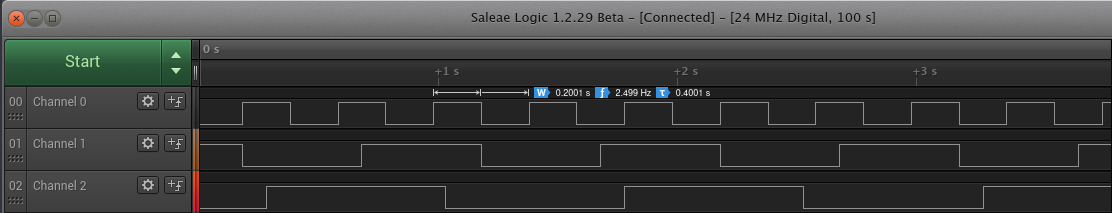
\includegraphics[scale=0.43]{img/SystickScheduler.png}

\caption{Saleae logic analyzer trace after the program ran free for a couple of seconds}
\label{fig:systick_sched_ver}

\end{figure}

The yellow LED is logic high for 0.5001 seconds and the green LED is logic high for 0.7502 seconds.
One can conclude that the timing specifications in Table \ref{tab:led_schedule} are met.
